% Options for packages loaded elsewhere
\PassOptionsToPackage{unicode}{hyperref}
\PassOptionsToPackage{hyphens}{url}
\PassOptionsToPackage{dvipsnames,svgnames,x11names}{xcolor}
%
\documentclass[
  letterpaper,
  DIV=11,
  numbers=noendperiod]{scrreprt}

\usepackage{amsmath,amssymb}
\usepackage{iftex}
\ifPDFTeX
  \usepackage[T1]{fontenc}
  \usepackage[utf8]{inputenc}
  \usepackage{textcomp} % provide euro and other symbols
\else % if luatex or xetex
  \usepackage{unicode-math}
  \defaultfontfeatures{Scale=MatchLowercase}
  \defaultfontfeatures[\rmfamily]{Ligatures=TeX,Scale=1}
\fi
\usepackage{lmodern}
\ifPDFTeX\else  
    % xetex/luatex font selection
\fi
% Use upquote if available, for straight quotes in verbatim environments
\IfFileExists{upquote.sty}{\usepackage{upquote}}{}
\IfFileExists{microtype.sty}{% use microtype if available
  \usepackage[]{microtype}
  \UseMicrotypeSet[protrusion]{basicmath} % disable protrusion for tt fonts
}{}
\makeatletter
\@ifundefined{KOMAClassName}{% if non-KOMA class
  \IfFileExists{parskip.sty}{%
    \usepackage{parskip}
  }{% else
    \setlength{\parindent}{0pt}
    \setlength{\parskip}{6pt plus 2pt minus 1pt}}
}{% if KOMA class
  \KOMAoptions{parskip=half}}
\makeatother
\usepackage{xcolor}
\setlength{\emergencystretch}{3em} % prevent overfull lines
\setcounter{secnumdepth}{5}
% Make \paragraph and \subparagraph free-standing
\makeatletter
\ifx\paragraph\undefined\else
  \let\oldparagraph\paragraph
  \renewcommand{\paragraph}{
    \@ifstar
      \xxxParagraphStar
      \xxxParagraphNoStar
  }
  \newcommand{\xxxParagraphStar}[1]{\oldparagraph*{#1}\mbox{}}
  \newcommand{\xxxParagraphNoStar}[1]{\oldparagraph{#1}\mbox{}}
\fi
\ifx\subparagraph\undefined\else
  \let\oldsubparagraph\subparagraph
  \renewcommand{\subparagraph}{
    \@ifstar
      \xxxSubParagraphStar
      \xxxSubParagraphNoStar
  }
  \newcommand{\xxxSubParagraphStar}[1]{\oldsubparagraph*{#1}\mbox{}}
  \newcommand{\xxxSubParagraphNoStar}[1]{\oldsubparagraph{#1}\mbox{}}
\fi
\makeatother

\usepackage{color}
\usepackage{fancyvrb}
\newcommand{\VerbBar}{|}
\newcommand{\VERB}{\Verb[commandchars=\\\{\}]}
\DefineVerbatimEnvironment{Highlighting}{Verbatim}{commandchars=\\\{\}}
% Add ',fontsize=\small' for more characters per line
\usepackage{framed}
\definecolor{shadecolor}{RGB}{241,243,245}
\newenvironment{Shaded}{\begin{snugshade}}{\end{snugshade}}
\newcommand{\AlertTok}[1]{\textcolor[rgb]{0.68,0.00,0.00}{#1}}
\newcommand{\AnnotationTok}[1]{\textcolor[rgb]{0.37,0.37,0.37}{#1}}
\newcommand{\AttributeTok}[1]{\textcolor[rgb]{0.40,0.45,0.13}{#1}}
\newcommand{\BaseNTok}[1]{\textcolor[rgb]{0.68,0.00,0.00}{#1}}
\newcommand{\BuiltInTok}[1]{\textcolor[rgb]{0.00,0.23,0.31}{#1}}
\newcommand{\CharTok}[1]{\textcolor[rgb]{0.13,0.47,0.30}{#1}}
\newcommand{\CommentTok}[1]{\textcolor[rgb]{0.37,0.37,0.37}{#1}}
\newcommand{\CommentVarTok}[1]{\textcolor[rgb]{0.37,0.37,0.37}{\textit{#1}}}
\newcommand{\ConstantTok}[1]{\textcolor[rgb]{0.56,0.35,0.01}{#1}}
\newcommand{\ControlFlowTok}[1]{\textcolor[rgb]{0.00,0.23,0.31}{\textbf{#1}}}
\newcommand{\DataTypeTok}[1]{\textcolor[rgb]{0.68,0.00,0.00}{#1}}
\newcommand{\DecValTok}[1]{\textcolor[rgb]{0.68,0.00,0.00}{#1}}
\newcommand{\DocumentationTok}[1]{\textcolor[rgb]{0.37,0.37,0.37}{\textit{#1}}}
\newcommand{\ErrorTok}[1]{\textcolor[rgb]{0.68,0.00,0.00}{#1}}
\newcommand{\ExtensionTok}[1]{\textcolor[rgb]{0.00,0.23,0.31}{#1}}
\newcommand{\FloatTok}[1]{\textcolor[rgb]{0.68,0.00,0.00}{#1}}
\newcommand{\FunctionTok}[1]{\textcolor[rgb]{0.28,0.35,0.67}{#1}}
\newcommand{\ImportTok}[1]{\textcolor[rgb]{0.00,0.46,0.62}{#1}}
\newcommand{\InformationTok}[1]{\textcolor[rgb]{0.37,0.37,0.37}{#1}}
\newcommand{\KeywordTok}[1]{\textcolor[rgb]{0.00,0.23,0.31}{\textbf{#1}}}
\newcommand{\NormalTok}[1]{\textcolor[rgb]{0.00,0.23,0.31}{#1}}
\newcommand{\OperatorTok}[1]{\textcolor[rgb]{0.37,0.37,0.37}{#1}}
\newcommand{\OtherTok}[1]{\textcolor[rgb]{0.00,0.23,0.31}{#1}}
\newcommand{\PreprocessorTok}[1]{\textcolor[rgb]{0.68,0.00,0.00}{#1}}
\newcommand{\RegionMarkerTok}[1]{\textcolor[rgb]{0.00,0.23,0.31}{#1}}
\newcommand{\SpecialCharTok}[1]{\textcolor[rgb]{0.37,0.37,0.37}{#1}}
\newcommand{\SpecialStringTok}[1]{\textcolor[rgb]{0.13,0.47,0.30}{#1}}
\newcommand{\StringTok}[1]{\textcolor[rgb]{0.13,0.47,0.30}{#1}}
\newcommand{\VariableTok}[1]{\textcolor[rgb]{0.07,0.07,0.07}{#1}}
\newcommand{\VerbatimStringTok}[1]{\textcolor[rgb]{0.13,0.47,0.30}{#1}}
\newcommand{\WarningTok}[1]{\textcolor[rgb]{0.37,0.37,0.37}{\textit{#1}}}

\providecommand{\tightlist}{%
  \setlength{\itemsep}{0pt}\setlength{\parskip}{0pt}}\usepackage{longtable,booktabs,array}
\usepackage{calc} % for calculating minipage widths
% Correct order of tables after \paragraph or \subparagraph
\usepackage{etoolbox}
\makeatletter
\patchcmd\longtable{\par}{\if@noskipsec\mbox{}\fi\par}{}{}
\makeatother
% Allow footnotes in longtable head/foot
\IfFileExists{footnotehyper.sty}{\usepackage{footnotehyper}}{\usepackage{footnote}}
\makesavenoteenv{longtable}
\usepackage{graphicx}
\makeatletter
\newsavebox\pandoc@box
\newcommand*\pandocbounded[1]{% scales image to fit in text height/width
  \sbox\pandoc@box{#1}%
  \Gscale@div\@tempa{\textheight}{\dimexpr\ht\pandoc@box+\dp\pandoc@box\relax}%
  \Gscale@div\@tempb{\linewidth}{\wd\pandoc@box}%
  \ifdim\@tempb\p@<\@tempa\p@\let\@tempa\@tempb\fi% select the smaller of both
  \ifdim\@tempa\p@<\p@\scalebox{\@tempa}{\usebox\pandoc@box}%
  \else\usebox{\pandoc@box}%
  \fi%
}
% Set default figure placement to htbp
\def\fps@figure{htbp}
\makeatother

\KOMAoption{captions}{tableheading}
\makeatletter
\@ifpackageloaded{tcolorbox}{}{\usepackage[skins,breakable]{tcolorbox}}
\@ifpackageloaded{fontawesome5}{}{\usepackage{fontawesome5}}
\definecolor{quarto-callout-color}{HTML}{909090}
\definecolor{quarto-callout-note-color}{HTML}{0758E5}
\definecolor{quarto-callout-important-color}{HTML}{CC1914}
\definecolor{quarto-callout-warning-color}{HTML}{EB9113}
\definecolor{quarto-callout-tip-color}{HTML}{00A047}
\definecolor{quarto-callout-caution-color}{HTML}{FC5300}
\definecolor{quarto-callout-color-frame}{HTML}{acacac}
\definecolor{quarto-callout-note-color-frame}{HTML}{4582ec}
\definecolor{quarto-callout-important-color-frame}{HTML}{d9534f}
\definecolor{quarto-callout-warning-color-frame}{HTML}{f0ad4e}
\definecolor{quarto-callout-tip-color-frame}{HTML}{02b875}
\definecolor{quarto-callout-caution-color-frame}{HTML}{fd7e14}
\makeatother
\makeatletter
\@ifpackageloaded{bookmark}{}{\usepackage{bookmark}}
\makeatother
\makeatletter
\@ifpackageloaded{caption}{}{\usepackage{caption}}
\AtBeginDocument{%
\ifdefined\contentsname
  \renewcommand*\contentsname{Table of contents}
\else
  \newcommand\contentsname{Table of contents}
\fi
\ifdefined\listfigurename
  \renewcommand*\listfigurename{List of Figures}
\else
  \newcommand\listfigurename{List of Figures}
\fi
\ifdefined\listtablename
  \renewcommand*\listtablename{List of Tables}
\else
  \newcommand\listtablename{List of Tables}
\fi
\ifdefined\figurename
  \renewcommand*\figurename{Figure}
\else
  \newcommand\figurename{Figure}
\fi
\ifdefined\tablename
  \renewcommand*\tablename{Table}
\else
  \newcommand\tablename{Table}
\fi
}
\@ifpackageloaded{float}{}{\usepackage{float}}
\floatstyle{ruled}
\@ifundefined{c@chapter}{\newfloat{codelisting}{h}{lop}}{\newfloat{codelisting}{h}{lop}[chapter]}
\floatname{codelisting}{Listing}
\newcommand*\listoflistings{\listof{codelisting}{List of Listings}}
\makeatother
\makeatletter
\makeatother
\makeatletter
\@ifpackageloaded{caption}{}{\usepackage{caption}}
\@ifpackageloaded{subcaption}{}{\usepackage{subcaption}}
\makeatother

\usepackage{bookmark}

\IfFileExists{xurl.sty}{\usepackage{xurl}}{} % add URL line breaks if available
\urlstyle{same} % disable monospaced font for URLs
\hypersetup{
  pdftitle={R Vignettes for Computational Social Science},
  pdfauthor={Daulton Selke},
  colorlinks=true,
  linkcolor={blue},
  filecolor={Maroon},
  citecolor={Blue},
  urlcolor={Blue},
  pdfcreator={LaTeX via pandoc}}


\title{R Vignettes for Computational Social Science}
\author{Daulton Selke}
\date{2025-09-10}

\begin{document}
\maketitle

\renewcommand*\contentsname{Table of contents}
{
\hypersetup{linkcolor=}
\setcounter{tocdepth}{2}
\tableofcontents
}

\bookmarksetup{startatroot}

\chapter*{Preface}\label{preface}
\addcontentsline{toc}{chapter}{Preface}

\markboth{Preface}{Preface}

Welcome! This page is currently under construction, but please enjoy
some of my instructional vignettes for various computational methods in
sociology and sociolinguistics.

\bookmarksetup{startatroot}

\chapter{Word Embeddings with US Federal Job
Advertisements}\label{word-embeddings-with-us-federal-job-advertisements}

The following code reproduces components of the analysis for the
in-progress manuscript, ``Occupational Segregation and Gendered Language
in Job Advertisements''

This project investigates whether and to what extent the gendered
composition of the federal workforce is associated with the amount of
gender stereotypical language in federal job advertisements, and, if so,
whether this relationship holds across different organizational
climates.

Our data comprises 5,526 job ads scraped at a single timepoint from the
US federal job-posting site USAJobs.gov, along with a number of
occupational characteristics imported from other sources such as the
Current Population Survey, O*NET, The Federal Employee Viewpoint Survey,
and the Survey on the Future of Government Service.

We conceptualize stereotype language in terms of social psycholoy's
Stereotype Content Model
\href{https://www.sciencedirect.com/science/article/pii/S0065260107000020?casa_token=HABSzi8Y7JMAAAAA:LBi45HX4KWxLfP4LLjsP8ySkpW1JtcZBNl67r55dZjmKbzsggVNarS--N6Y9XWdcn_q3zGfTI_c}{(Cuddy,
Fiske, and Glick 2008)}. To operationalize the stereotype content model,
we utilized word embeddings in conjunction with
\href{https://link.springer.com/article/10.1007/s42001-019-00048-6}{Stoltz
and Taylor's (2019)} Concept Mover's Distance as an instrument for
measuring the degree of warmth- and competence-language across job ads.

\section{Setting up the Workspace}\label{setting-up-the-workspace}

Let's load some packages

\begin{verbatim}
Skipping install of 'text2map.pretrained' from a gitlab remote, the SHA1 (f17fbff7) has not changed since last install.
  Use `force = TRUE` to force installation
\end{verbatim}

\begin{Shaded}
\begin{Highlighting}[]
\FunctionTok{library}\NormalTok{(ggrepel)}
\FunctionTok{library}\NormalTok{(text2map)}
\FunctionTok{library}\NormalTok{(text2vec)}
\FunctionTok{library}\NormalTok{(gutenbergr)}
\FunctionTok{library}\NormalTok{(tidyverse)}
\FunctionTok{library}\NormalTok{(textclean)}
\FunctionTok{library}\NormalTok{(stringi)}
\FunctionTok{library}\NormalTok{(text2map.pretrained)}
\FunctionTok{library}\NormalTok{(flextable)}
\FunctionTok{library}\NormalTok{(huxtable)}
\FunctionTok{library}\NormalTok{(sjPlot)}
\FunctionTok{library}\NormalTok{(interactions)}
\FunctionTok{library}\NormalTok{(remotes)}
\end{Highlighting}
\end{Shaded}

You might have to install a couple of these, but all of them can be
installed with \texttt{install.packages()} except for
\texttt{text2map.pretrained}, so go ahead and download that with the
following command

\begin{Shaded}
\begin{Highlighting}[]
\NormalTok{remotes}\SpecialCharTok{::}\FunctionTok{install\_gitlab}\NormalTok{(}\StringTok{"culturalcartography/text2map.pretrained"}\NormalTok{)}
\end{Highlighting}
\end{Shaded}

Now, go ahead and load ``workingjobs.df'' into your workspace. You can
use \texttt{file.choose()} with \texttt{load()} to pull up a
file-explorer window and manually select the data.

\begin{Shaded}
\begin{Highlighting}[]
\FunctionTok{load}\NormalTok{(}\FunctionTok{file.choose}\NormalTok{())}
\end{Highlighting}
\end{Shaded}

We also need to download our pre-trained vector embeddings. We use
\href{https://fasttext.cc/docs/en/english-vectors.html}{fastText
embeddings}, which are trained on a large corpus of English Wikipedia
and various news data sets. This way, our embeddings will reflect a
sense of public meaning. This works well for many research questions,
but you may want to consider training your own embeddings in the event
that your data is stylistically unique.

\begin{tcolorbox}[enhanced jigsaw, title=\textcolor{quarto-callout-caution-color}{\faFire}\hspace{0.5em}{Caution}, colbacktitle=quarto-callout-caution-color!10!white, left=2mm, opacityback=0, colback=white, coltitle=black, toprule=.15mm, opacitybacktitle=0.6, breakable, colframe=quarto-callout-caution-color-frame, rightrule=.15mm, toptitle=1mm, bottomtitle=1mm, titlerule=0mm, arc=.35mm, leftrule=.75mm, bottomrule=.15mm]

The fastText embeddings file is very large. It will be over a gigabyte,
so keep that in mind before you download. You only have to run the
following command once ever, so consider commenting it out of your
script after you do so. You don't want to keep downloading such a huge
file by mistake.

\end{tcolorbox}

\begin{Shaded}
\begin{Highlighting}[]
\FunctionTok{download\_pretrained}\NormalTok{(}\StringTok{"vecs\_fasttext300\_wiki\_news"}\NormalTok{)}
\end{Highlighting}
\end{Shaded}

After that finishes downloading, go ahead and load the embeddings object
in. You will want to do this anytime you work with your embeddings. It
won't download anything new---it just retrieves the file you downloaded
with the command above.

\begin{Shaded}
\begin{Highlighting}[]
\FunctionTok{data}\NormalTok{(}\StringTok{"vecs\_fasttext300\_wiki\_news"}\NormalTok{)}
\NormalTok{our\_wv}\OtherTok{\textless{}{-}}\NormalTok{vecs\_fasttext300\_wiki\_news}
\FunctionTok{rm}\NormalTok{(vecs\_fasttext300\_wiki\_news)}
\end{Highlighting}
\end{Shaded}

Because the file name is a bit cumbersome, Stoltz \& Taylor recommend
renaming the object and then removing the original file.

\section{Calculating our Response Variable with Concept Mover's
Distance}\label{calculating-our-response-variable-with-concept-movers-distance}

Below, we will use pre-trained vector encodings to calculate the Concept
Mover's Distance for stereotype content language across all of our job
ads. Note that much of this section makes heavy use of the excellent
\href{https://culturalcartography.gitlab.io/text2map/}{text2map} package
from
\href{https://global.oup.com/academic/product/mapping-texts-9780197756881?cc=us&lang=en&}{Stoltz
and Taylor (2023)}.

\subsection{Wrangle our Embeddings}\label{wrangle-our-embeddings}

First, we'll borrow some code from \emph{Mapping Texts} to build a
document-term matrix. This will give us a new dataframe where each row
is a document, each column is a single word, and each cell reflects the
count of some word in a given document.

\begin{Shaded}
\begin{Highlighting}[]
\NormalTok{dtm\_ja }\OtherTok{\textless{}{-}}\NormalTok{ workingjobs.df }\SpecialCharTok{|\textgreater{}}
  \FunctionTok{dtm\_builder}\NormalTok{(string\_lemma, doc\_id) }\SpecialCharTok{|\textgreater{}}
  \FunctionTok{dtm\_stopper}\NormalTok{(}\AttributeTok{stop\_list =} \FunctionTok{get\_stoplist}\NormalTok{(}\StringTok{"snowball2014"}\NormalTok{),}
              \AttributeTok{stop\_docprop =} \FunctionTok{c}\NormalTok{(.}\DecValTok{01}\NormalTok{, }\ConstantTok{Inf}\NormalTok{))}
\end{Highlighting}
\end{Shaded}

\texttt{string\_lemma} is the column that contains our job ad text after
various pre-processing procedures. Note that we are also removing a list
of common stop words, using the predefined Snowball list. Stop words are
typically function words that occur with high frequency. For cultural
measurement of text data, we are often more interested in content words
that bare more straightforward semantic information, so including stop
words can muddy our instrument. Lastly, we use \texttt{stop\_docprop} to
set a low-end exclusion criteria for word frequency. Any word that
appears in less than 1\% of all documents will be dropped from our DTM.

Now, let's take a subset of the word embeddings object. We want an
object that includes the vector embeddings for only the words in our
cleaned DTM. Remember that the columns of the DTM are words in the job
ads corpus, and the row names of \texttt{our\_wv} are all 1 million
words in the pre-trained embeddings. We can use this to subset.

\begin{Shaded}
\begin{Highlighting}[]
\NormalTok{job\_vectors }\OtherTok{\textless{}{-}}\NormalTok{ our\_wv[}\FunctionTok{rownames}\NormalTok{(our\_wv) }\SpecialCharTok{\%in\%} \FunctionTok{colnames}\NormalTok{(dtm\_ja), ]}
\end{Highlighting}
\end{Shaded}

\subsection{Mapping Warmth and
Competence}\label{mapping-warmth-and-competence}

For Concept Mover's Distance, we need two word lists reflecting each of
our two oppositional concepts of interest. Let's load in our paired
lists of warmth and competence words. Note that we derived these pairs
from the warmth/competence seed dictionary created by
\href{https://onlinelibrary.wiley.com/doi/full/10.1002/ejsp.2724?casa_token=gqMHBVmq7eUAAAAA\%3Azr6pilqgfE2nbpJ6yt1aikGXx4GZnenVpTp3F6g9kEPglQqBvFedzgMtbFPuH0mVQ1JUUkzgitZeR6M}{Gandalf,
Bai, and Fiske's (2020)}.

\begin{Shaded}
\begin{Highlighting}[]
\FunctionTok{load}\NormalTok{(}\FunctionTok{file.choose}\NormalTok{())}
\end{Highlighting}
\end{Shaded}

Go ahead and load in ``scm\_antonym\_pairs.csv''

Now we will calculate a semantic direction using our paired wordlist and
our original word embedding object, \texttt{our\_wv}. The semantic
direction is the difference of the two vectors, which gives us the pole
between the warmth and competence regions we defined in embedding space.

Then, we'll use the semantic direction to generate the Concept Mover's
Distance for each job. You can refer to Stoltz \& Taylor's original
paper on this for more details on the calculation, but it essentially
maps each document along the semantic direction pole. This will allow us
to estimate how close the vector space of each job ad is to the
competence region vs.~the warmth region. This gives us our measure of
conceptual prominence.

\begin{Shaded}
\begin{Highlighting}[]
\NormalTok{sd\_stereo }\OtherTok{\textless{}{-}} \FunctionTok{get\_direction}\NormalTok{(scm\_ant, our\_wv, }\AttributeTok{method=}\StringTok{"paired"}\NormalTok{)}
\NormalTok{closeness }\OtherTok{\textless{}{-}} \FunctionTok{CMDist}\NormalTok{(}\AttributeTok{dtm=}\NormalTok{ dtm\_ja, }\AttributeTok{cv =}\NormalTok{ sd\_stereo, }\AttributeTok{wv =}\NormalTok{ job\_vectors)}
\end{Highlighting}
\end{Shaded}

The \texttt{closeness} object will be a 2-column data frame including
the Concept Mover's Distance scores for each ad and the \texttt{doc\_id}
column, which we can use to merge these values into our job ads data
frame.

Because of the way we set up our paired wordlist, positive values
reflect more engagement with competence language, and negative values
reflect more warmth engagement.

Note that it will name the CMD column with the format \texttt{*\_pole},
where \texttt{*} is a stand-in for the first word on the left-side of
our wordlist of warmth/competence pairs. That will be `ability' in our
case, so let's rename it something more descriptive.

\begin{Shaded}
\begin{Highlighting}[]
\FunctionTok{names}\NormalTok{(closeness)[}\DecValTok{2}\NormalTok{]}\OtherTok{\textless{}{-}}\StringTok{"comp\_warm\_scale"}
\end{Highlighting}
\end{Shaded}

Now, we can merge these values into our original data frame.

\begin{Shaded}
\begin{Highlighting}[]
\NormalTok{workingjobs.df }\OtherTok{\textless{}{-}} \FunctionTok{merge}\NormalTok{(workingjobs.df, closeness)}
\end{Highlighting}
\end{Shaded}

\subsection{View the Warmest and Most Competence
Words}\label{view-the-warmest-and-most-competence-words}

Now we've got our measure of warmth/competence prominence! There's
plenty more we can do with embeddings, but we are winding down the
current tutorial.

I'll leave you with one last neat example highlighted in \emph{Mapping
Texts} I will borrow some more code from Stoltz and Taylor to show you
how you can view the individual words whose vector embeddings were
closest to warmth or competence. CMD is a document level measure, but we
can do all kinds of fun stuff with individual embeddings. Below are the
words estimated to most strongly engage one concept or the other.

\begin{Shaded}
\begin{Highlighting}[]
\NormalTok{comp\_warm }\OtherTok{\textless{}{-}} \FunctionTok{get\_direction}\NormalTok{(}\AttributeTok{anchors =}\NormalTok{ scm\_ant, }\AttributeTok{wv =}\NormalTok{ our\_wv, }\AttributeTok{method=}\StringTok{"paired"}\NormalTok{)}

\FunctionTok{row.names}\NormalTok{(comp\_warm)[}\DecValTok{1}\NormalTok{]}\OtherTok{\textless{}{-}}\StringTok{"competence\_pole"}

\NormalTok{sim\_dir }\OtherTok{\textless{}{-}} \FunctionTok{sim2}\NormalTok{(comp\_warm, job\_vectors, }\AttributeTok{method =} \StringTok{"cosine"}\NormalTok{)}
\NormalTok{df\_dir }\OtherTok{\textless{}{-}} \FunctionTok{data.frame}\NormalTok{(}\AttributeTok{competence\_pole =}\NormalTok{ sim\_dir[}\StringTok{"competence\_pole"}\NormalTok{, ],}
                     \AttributeTok{terms =} \FunctionTok{colnames}\NormalTok{(sim\_dir)) }\SpecialCharTok{|\textgreater{}}
  \FunctionTok{mutate}\NormalTok{(}\AttributeTok{comp\_warm\_label =} \FunctionTok{ifelse}\NormalTok{(}
\NormalTok{    competence\_pole }\SpecialCharTok{\textgreater{}=} \DecValTok{0}\NormalTok{,}
    \StringTok{"Competence"}\NormalTok{, }\StringTok{"Warmth"}\NormalTok{),}
    \AttributeTok{comp\_warm =} \FunctionTok{abs}\NormalTok{(competence\_pole)}
\NormalTok{  )}

\NormalTok{df\_dir }\SpecialCharTok{|\textgreater{}}
  \FunctionTok{group\_by}\NormalTok{(comp\_warm\_label) }\SpecialCharTok{|\textgreater{}}
  \FunctionTok{slice\_max}\NormalTok{(comp\_warm, }\AttributeTok{n =} \DecValTok{30}\NormalTok{) }\SpecialCharTok{|\textgreater{}}
  \FunctionTok{mutate}\NormalTok{(}\AttributeTok{term =} \FunctionTok{fct\_reorder}\NormalTok{(terms, comp\_warm)) }\SpecialCharTok{|\textgreater{}}
  \FunctionTok{ggplot}\NormalTok{(}\FunctionTok{aes}\NormalTok{(term, comp\_warm, }\AttributeTok{fill =}\NormalTok{ comp\_warm\_label, }\AttributeTok{label =}\NormalTok{ terms)) }\SpecialCharTok{+}
  \FunctionTok{geom\_col}\NormalTok{() }\SpecialCharTok{+}
  \FunctionTok{guides}\NormalTok{(}\AttributeTok{fill =} \StringTok{"none"}\NormalTok{) }\SpecialCharTok{+}
  \FunctionTok{labs}\NormalTok{(}\AttributeTok{x =} \ConstantTok{NULL}\NormalTok{, }\AttributeTok{y =} \StringTok{"Cosine Similarity to Pole"}\NormalTok{) }\SpecialCharTok{+}
  \FunctionTok{coord\_flip}\NormalTok{() }\SpecialCharTok{+}
  \FunctionTok{facet\_wrap}\NormalTok{(}\SpecialCharTok{\textasciitilde{}}\NormalTok{comp\_warm\_label, }\AttributeTok{scale =} \StringTok{"free"}\NormalTok{)}
\end{Highlighting}
\end{Shaded}

\pandocbounded{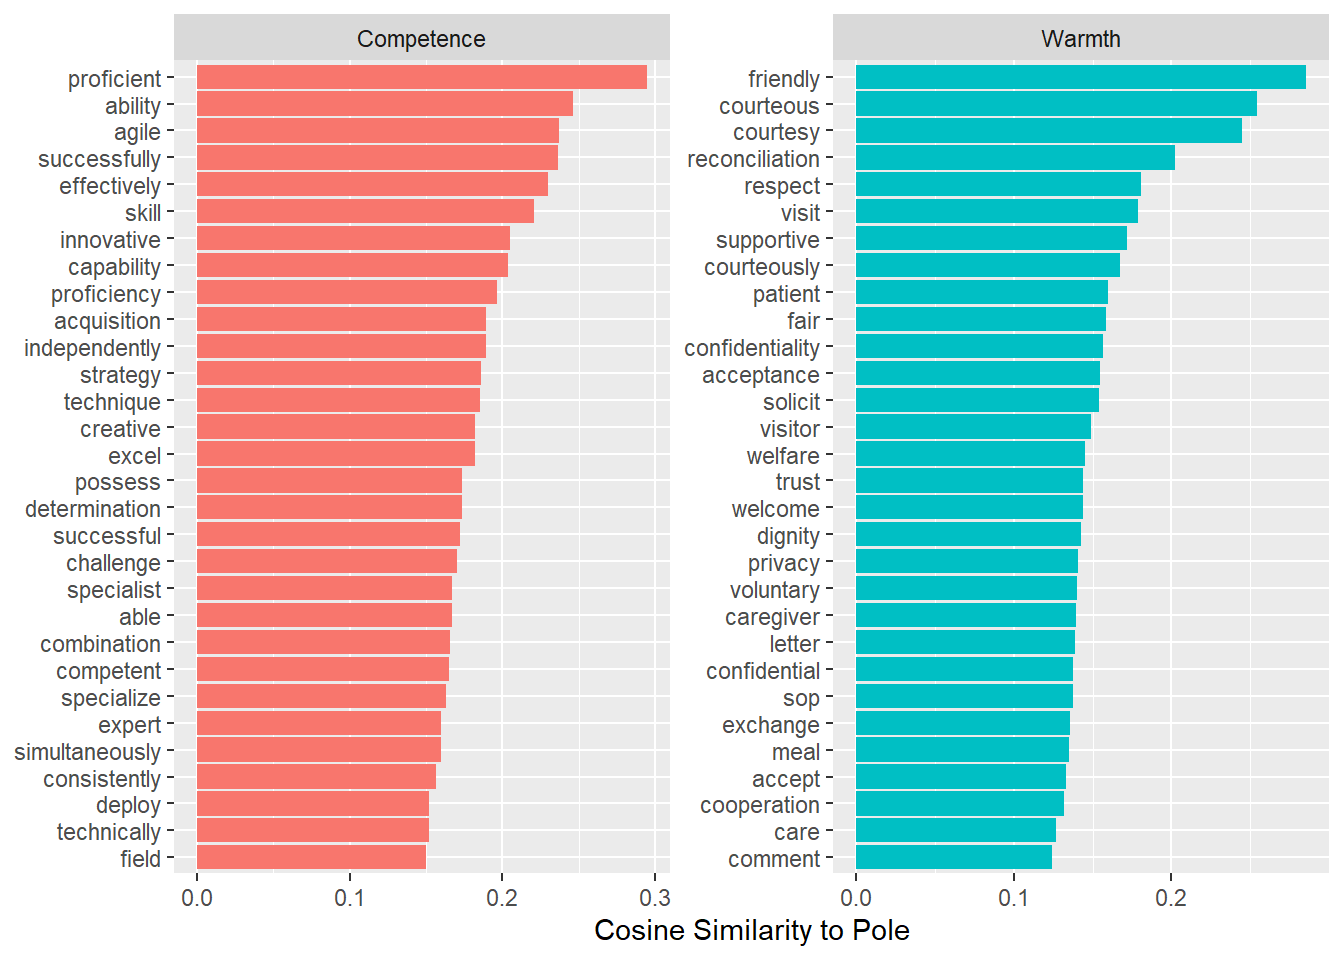
\includegraphics[keepaspectratio]{usajobs_embeddings_files/figure-pdf/unnamed-chunk-15-1.pdf}}




\end{document}
